% Options for packages loaded elsewhere
\PassOptionsToPackage{unicode}{hyperref}
\PassOptionsToPackage{hyphens}{url}
\PassOptionsToPackage{dvipsnames,svgnames*,x11names*}{xcolor}
%
\documentclass[
  9pt,
]{krantz}
\usepackage{lmodern}
\usepackage{amssymb,amsmath}
\usepackage{ifxetex,ifluatex}
\ifnum 0\ifxetex 1\fi\ifluatex 1\fi=0 % if pdftex
  \usepackage[T1]{fontenc}
  \usepackage[utf8]{inputenc}
  \usepackage{textcomp} % provide euro and other symbols
\else % if luatex or xetex
  \usepackage{unicode-math}
  \defaultfontfeatures{Scale=MatchLowercase}
  \defaultfontfeatures[\rmfamily]{Ligatures=TeX,Scale=1}
  \setmonofont[Scale=0.7]{Source Code Pro}
\fi
% Use upquote if available, for straight quotes in verbatim environments
\IfFileExists{upquote.sty}{\usepackage{upquote}}{}
\IfFileExists{microtype.sty}{% use microtype if available
  \usepackage[]{microtype}
  \UseMicrotypeSet[protrusion]{basicmath} % disable protrusion for tt fonts
}{}
\makeatletter
\@ifundefined{KOMAClassName}{% if non-KOMA class
  \IfFileExists{parskip.sty}{%
    \usepackage{parskip}
  }{% else
    \setlength{\parindent}{0pt}
    \setlength{\parskip}{6pt plus 2pt minus 1pt}}
}{% if KOMA class
  \KOMAoptions{parskip=half}}
\makeatother
\usepackage{xcolor}
\IfFileExists{xurl.sty}{\usepackage{xurl}}{} % add URL line breaks if available
\IfFileExists{bookmark.sty}{\usepackage{bookmark}}{\usepackage{hyperref}}
\hypersetup{
  pdftitle={R로 하는 약동학 모델링},
  pdfauthor={한성필},
  colorlinks=true,
  linkcolor=Maroon,
  filecolor=Maroon,
  citecolor=Blue,
  urlcolor=Blue,
  pdfcreator={LaTeX via pandoc}}
\urlstyle{same} % disable monospaced font for URLs
\usepackage{color}
\usepackage{fancyvrb}
\newcommand{\VerbBar}{|}
\newcommand{\VERB}{\Verb[commandchars=\\\{\}]}
\DefineVerbatimEnvironment{Highlighting}{Verbatim}{commandchars=\\\{\}}
% Add ',fontsize=\small' for more characters per line
\usepackage{framed}
\definecolor{shadecolor}{RGB}{248,248,248}
\newenvironment{Shaded}{\begin{snugshade}}{\end{snugshade}}
\newcommand{\AlertTok}[1]{\textcolor[rgb]{0.94,0.16,0.16}{#1}}
\newcommand{\AnnotationTok}[1]{\textcolor[rgb]{0.56,0.35,0.01}{\textbf{\textit{#1}}}}
\newcommand{\AttributeTok}[1]{\textcolor[rgb]{0.77,0.63,0.00}{#1}}
\newcommand{\BaseNTok}[1]{\textcolor[rgb]{0.00,0.00,0.81}{#1}}
\newcommand{\BuiltInTok}[1]{#1}
\newcommand{\CharTok}[1]{\textcolor[rgb]{0.31,0.60,0.02}{#1}}
\newcommand{\CommentTok}[1]{\textcolor[rgb]{0.56,0.35,0.01}{\textit{#1}}}
\newcommand{\CommentVarTok}[1]{\textcolor[rgb]{0.56,0.35,0.01}{\textbf{\textit{#1}}}}
\newcommand{\ConstantTok}[1]{\textcolor[rgb]{0.00,0.00,0.00}{#1}}
\newcommand{\ControlFlowTok}[1]{\textcolor[rgb]{0.13,0.29,0.53}{\textbf{#1}}}
\newcommand{\DataTypeTok}[1]{\textcolor[rgb]{0.13,0.29,0.53}{#1}}
\newcommand{\DecValTok}[1]{\textcolor[rgb]{0.00,0.00,0.81}{#1}}
\newcommand{\DocumentationTok}[1]{\textcolor[rgb]{0.56,0.35,0.01}{\textbf{\textit{#1}}}}
\newcommand{\ErrorTok}[1]{\textcolor[rgb]{0.64,0.00,0.00}{\textbf{#1}}}
\newcommand{\ExtensionTok}[1]{#1}
\newcommand{\FloatTok}[1]{\textcolor[rgb]{0.00,0.00,0.81}{#1}}
\newcommand{\FunctionTok}[1]{\textcolor[rgb]{0.00,0.00,0.00}{#1}}
\newcommand{\ImportTok}[1]{#1}
\newcommand{\InformationTok}[1]{\textcolor[rgb]{0.56,0.35,0.01}{\textbf{\textit{#1}}}}
\newcommand{\KeywordTok}[1]{\textcolor[rgb]{0.13,0.29,0.53}{\textbf{#1}}}
\newcommand{\NormalTok}[1]{#1}
\newcommand{\OperatorTok}[1]{\textcolor[rgb]{0.81,0.36,0.00}{\textbf{#1}}}
\newcommand{\OtherTok}[1]{\textcolor[rgb]{0.56,0.35,0.01}{#1}}
\newcommand{\PreprocessorTok}[1]{\textcolor[rgb]{0.56,0.35,0.01}{\textit{#1}}}
\newcommand{\RegionMarkerTok}[1]{#1}
\newcommand{\SpecialCharTok}[1]{\textcolor[rgb]{0.00,0.00,0.00}{#1}}
\newcommand{\SpecialStringTok}[1]{\textcolor[rgb]{0.31,0.60,0.02}{#1}}
\newcommand{\StringTok}[1]{\textcolor[rgb]{0.31,0.60,0.02}{#1}}
\newcommand{\VariableTok}[1]{\textcolor[rgb]{0.00,0.00,0.00}{#1}}
\newcommand{\VerbatimStringTok}[1]{\textcolor[rgb]{0.31,0.60,0.02}{#1}}
\newcommand{\WarningTok}[1]{\textcolor[rgb]{0.56,0.35,0.01}{\textbf{\textit{#1}}}}
\usepackage{longtable,booktabs}
% Correct order of tables after \paragraph or \subparagraph
\usepackage{etoolbox}
\makeatletter
\patchcmd\longtable{\par}{\if@noskipsec\mbox{}\fi\par}{}{}
\makeatother
% Allow footnotes in longtable head/foot
\IfFileExists{footnotehyper.sty}{\usepackage{footnotehyper}}{\usepackage{footnote}}
\makesavenoteenv{longtable}
\usepackage{graphicx,grffile}
\makeatletter
\def\maxwidth{\ifdim\Gin@nat@width>\linewidth\linewidth\else\Gin@nat@width\fi}
\def\maxheight{\ifdim\Gin@nat@height>\textheight\textheight\else\Gin@nat@height\fi}
\makeatother
% Scale images if necessary, so that they will not overflow the page
% margins by default, and it is still possible to overwrite the defaults
% using explicit options in \includegraphics[width, height, ...]{}
\setkeys{Gin}{width=\maxwidth,height=\maxheight,keepaspectratio}
% Set default figure placement to htbp
\makeatletter
\def\fps@figure{htbp}
\makeatother
\setlength{\emergencystretch}{3em} % prevent overfull lines
\providecommand{\tightlist}{%
  \setlength{\itemsep}{0pt}\setlength{\parskip}{0pt}}
\setcounter{secnumdepth}{5}
\usepackage{kotex}

\title{R로 하는 약동학 모델링}
\author{한성필}
\date{2019-11-07}

\begin{document}
\maketitle

{
\hypersetup{linkcolor=}
\setcounter{tocdepth}{2}
\tableofcontents
}
\listoftables
\listoffigures
\hypertarget{introduction}{%
\chapter*{Introduction}\label{introduction}}


이 자료는 Johan Gabrielsson과 Dan Weiner의 책, ``Pharmacokinetic and Pharmacodynamic Data Analysis - Concepts and Applications'' 5th ed.~(Gabrielsson \protect\hyperlink{ref-gab}{2016})를 풀기 위한 것입니다. 서울아산병원 임상약리학과 배균섭 교수님께서 개발한 \texttt{wnl}패키지 (Bae \protect\hyperlink{ref-R-wnl}{2018})를 활용하였습니다.

오탈자 신고 등은 \href{https://github.com/pipetcpt/study-pkpd/issues}{깃허브 저장소}에 남겨주십시오.

감사합니다.

2019년 11월\\
가톨릭대학교 약리학교실\\
연구강사 한성필

\mainmatter

\hypertarget{one-compartment-model---oral-dosing}{%
\chapter{One compartment model - oral dosing}\label{one-compartment-model---oral-dosing}}

\texttt{wnl} 라이브러리를 불러오고 자료를 읽어옵니다.

\begin{Shaded}
\begin{Highlighting}[]
\KeywordTok{library}\NormalTok{(wnl)}
\NormalTok{dPK02 =}\StringTok{ }\KeywordTok{read.csv}\NormalTok{(}\StringTok{"data/hands-on1.csv"}\NormalTok{, }\DataTypeTok{skip=}\DecValTok{1}\NormalTok{)}
\KeywordTok{colnames}\NormalTok{(dPK02) =}\StringTok{ }\KeywordTok{c}\NormalTok{(}\StringTok{"TIME"}\NormalTok{, }\StringTok{"DV"}\NormalTok{)}
\KeywordTok{plot}\NormalTok{(dPK02[,}\StringTok{"TIME"}\NormalTok{], dPK02[,}\StringTok{"DV"}\NormalTok{], }\DataTypeTok{xlim=}\KeywordTok{c}\NormalTok{(}\DecValTok{0}\NormalTok{, }\DecValTok{400}\NormalTok{), }\DataTypeTok{ylim=}\KeywordTok{c}\NormalTok{(}\DecValTok{0}\NormalTok{, }\FloatTok{2.5}\NormalTok{), }
     \DataTypeTok{xlab=}\StringTok{"Time (min)"}\NormalTok{, }\DataTypeTok{ylab=}\StringTok{"Concentration (ug/L)"}\NormalTok{, }\DataTypeTok{pch=}\DecValTok{16}\NormalTok{)}
\end{Highlighting}
\end{Shaded}

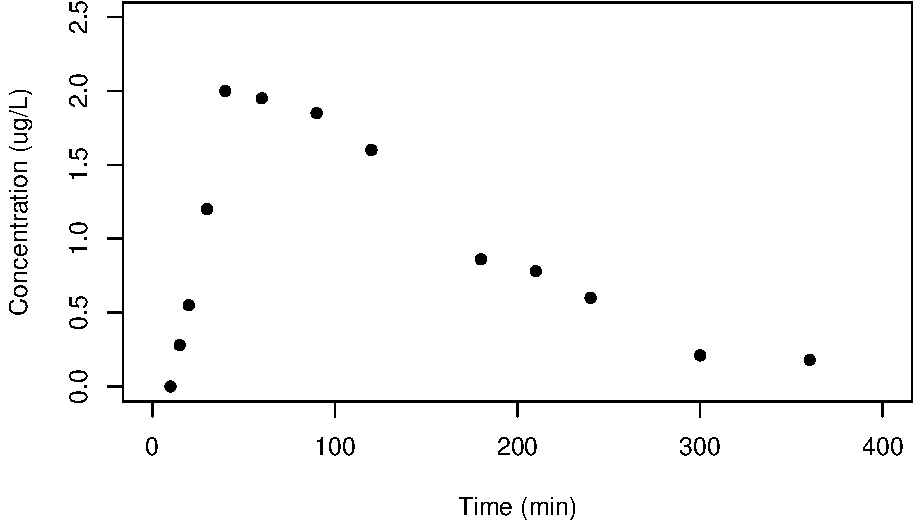
\includegraphics{handout_files/figure-latex/unnamed-chunk-1-1.pdf}

먼저 NCA 분석을 해 봅니다. Tmax는 40분, Cmax는 2.00 ug/L인 것을 알 수 있습니다.

\begin{Shaded}
\begin{Highlighting}[]
\NormalTok{NonCompart}\OperatorTok{::}\KeywordTok{sNCA}\NormalTok{(dPK02[,}\StringTok{"TIME"}\NormalTok{], dPK02[,}\StringTok{"DV"}\NormalTok{], }\DataTypeTok{dose=}\DecValTok{100}\NormalTok{, }\DataTypeTok{doseUnit=}\StringTok{"ug"}\NormalTok{, }\DataTypeTok{timeUnit=}\StringTok{"min"}\NormalTok{)}
\end{Highlighting}
\end{Shaded}

\begin{verbatim}
##            b0          CMAX         CMAXD          TMAX          TLAG 
##  1.557534e+00  2.000000e+00  2.000000e-02  4.000000e+01  1.000000e+01 
##          CLST         CLSTP          TLST        LAMZHL          LAMZ 
##  1.800000e-01  1.647689e-01  3.600000e+02  7.424929e+01  9.335405e-03 
##        LAMZLL        LAMZUL       LAMZNPT        CORRXY            R2 
##  9.000000e+01  3.600000e+02  7.000000e+00 -9.822141e-01  9.647446e-01 
##         R2ADJ        AUCLST        AUCALL        AUCIFO       AUCIFOD 
##  9.576935e-01  3.308750e+02  3.308750e+02  3.501564e+02  3.501564e+00 
##        AUCIFP       AUCIFPD        AUCPEO        AUCPEP       AUMCLST 
##  3.485249e+02  3.485249e+00  5.506520e+00  5.064170e+00  4.230750e+04 
##       AUMCIFO       AUMCIFP       AUMCPEO       AUMCPEP          VZFO 
##  5.131423e+04  5.055210e+04  1.755210e+01  1.630912e+01  3.059178e+01 
##          VZFP          CLFO          CLFP      MRTEVLST      MRTEVIFO 
##  3.073499e+01  2.855866e-01  2.869236e-01  1.278655e+02  1.465466e+02 
##      MRTEVIFP 
##  1.450459e+02 
## attr(,"units")
##  [1] ""            "ug/L"        "ug/L/ug"     "min"         "min"        
##  [6] "ug/L"        "ug/L"        "min"         "min"         "/min"       
## [11] "min"         "min"         ""            ""            ""           
## [16] ""            "min*ug/L"    "min*ug/L"    "min*ug/L"    "min*ug/L/ug"
## [21] "min*ug/L"    "min*ug/L/ug" "%"           "%"           "min2*ug/L"  
## [26] "min2*ug/L"   "min2*ug/L"   "%"           "%"           "L"          
## [31] "L"           "L/min"       "L/min"       "min"         "min"        
## [36] "min"        
## attr(,"UsedPoints")
## [1]  7  8  9 10 11 12 13
\end{verbatim}

\hypertarget{compartmental-analysis-without-tlag}{%
\section{Compartmental analysis without Tlag}\label{compartmental-analysis-without-tlag}}

경구 투여 일구획 분석, 지연시간이 없는 모형입니다. Ka, V, K로 농도를 나타낼 수 있습니다.

\begin{Shaded}
\begin{Highlighting}[]
\NormalTok{DOSE =}\StringTok{ }\DecValTok{100}

\NormalTok{fPK02a =}\StringTok{ }\ControlFlowTok{function}\NormalTok{(THETA) }\CommentTok{# Prediction function}
\NormalTok{\{}
\NormalTok{  Ka =}\StringTok{ }\NormalTok{THETA[}\DecValTok{1}\NormalTok{]}
\NormalTok{  V  =}\StringTok{ }\NormalTok{THETA[}\DecValTok{2}\NormalTok{]}
\NormalTok{  K  =}\StringTok{ }\NormalTok{THETA[}\DecValTok{3}\NormalTok{]}
\NormalTok{  Cp =}\StringTok{ }\NormalTok{DOSE}\OperatorTok{/}\NormalTok{V}\OperatorTok{*}\NormalTok{Ka}\OperatorTok{/}\NormalTok{(Ka }\OperatorTok{-}\StringTok{ }\NormalTok{K)}\OperatorTok{*}\NormalTok{(}\KeywordTok{exp}\NormalTok{(}\OperatorTok{-}\NormalTok{K}\OperatorTok{*}\NormalTok{TIME) }\OperatorTok{-}\StringTok{ }\KeywordTok{exp}\NormalTok{(}\OperatorTok{-}\NormalTok{Ka}\OperatorTok{*}\NormalTok{TIME)) }\CommentTok{# eq 2:1}
  \KeywordTok{return}\NormalTok{(Cp)}
\NormalTok{\}}
\NormalTok{TIME =}\StringTok{ }\NormalTok{dPK02[,}\StringTok{"TIME"}\NormalTok{]}
\NormalTok{r1 =}\StringTok{ }\KeywordTok{nlr}\NormalTok{(fPK02a, dPK02, }\DataTypeTok{pNames=}\KeywordTok{c}\NormalTok{(}\StringTok{"ka"}\NormalTok{, }\StringTok{"V"}\NormalTok{, }\StringTok{"k"}\NormalTok{), }\DataTypeTok{IE=}\KeywordTok{c}\NormalTok{(}\FloatTok{0.1}\NormalTok{, }\DecValTok{30}\NormalTok{, }\FloatTok{0.05}\NormalTok{))}

\NormalTok{r1}\OperatorTok{$}\NormalTok{Est}
\end{Highlighting}
\end{Shaded}

\begin{verbatim}
##               ka         V            k   AddErrVar    AddErrSD
## PE   0.013202142 21.017659  0.013202008  0.08701446  0.29498213
## SE   0.005442004  8.623411  0.005441954  0.03412981  0.05785063
## RSE 41.220611647 41.029360 41.220651532 39.22314350 19.61157175
\end{verbatim}

\hypertarget{compartmental-analysis-with-tlag}{%
\section{Compartmental analysis with Tlag}\label{compartmental-analysis-with-tlag}}

경구 투여 일구획 분석, 지연시간이 있는 모형입니다. Ka, V, K에 Tlag가 추가되어 농도를 나타낼 수 있습니다.

\begin{Shaded}
\begin{Highlighting}[]
\NormalTok{fPK02b =}\StringTok{ }\ControlFlowTok{function}\NormalTok{(THETA) }\CommentTok{# Prediction function}
\NormalTok{\{}
\NormalTok{  Ka   =}\StringTok{ }\NormalTok{THETA[}\DecValTok{1}\NormalTok{]}
\NormalTok{  V    =}\StringTok{ }\NormalTok{THETA[}\DecValTok{2}\NormalTok{]}
\NormalTok{  K    =}\StringTok{ }\NormalTok{THETA[}\DecValTok{3}\NormalTok{]}
\NormalTok{  tlag =}\StringTok{ }\NormalTok{THETA[}\DecValTok{4}\NormalTok{]}

\NormalTok{  Cp  =}\StringTok{ }\NormalTok{DOSE}\OperatorTok{/}\NormalTok{V}\OperatorTok{*}\NormalTok{Ka}\OperatorTok{/}\NormalTok{(Ka }\OperatorTok{-}\StringTok{ }\NormalTok{K)}\OperatorTok{*}\NormalTok{(}\KeywordTok{exp}\NormalTok{(}\OperatorTok{-}\NormalTok{K}\OperatorTok{*}\NormalTok{(TIME }\OperatorTok{-}\StringTok{ }\NormalTok{tlag)) }\OperatorTok{-}\StringTok{ }\KeywordTok{exp}\NormalTok{(}\OperatorTok{-}\NormalTok{Ka}\OperatorTok{*}\NormalTok{(TIME }\OperatorTok{-}\StringTok{ }\NormalTok{tlag))) }\CommentTok{# eq 2:2}
  \KeywordTok{return}\NormalTok{(Cp)}
\NormalTok{\}}
\NormalTok{TIME =}\StringTok{ }\NormalTok{dPK02[,}\StringTok{"TIME"}\NormalTok{]}
\NormalTok{r2 =}\StringTok{ }\KeywordTok{nlr}\NormalTok{(fPK02b, dPK02, }\DataTypeTok{pNames=}\KeywordTok{c}\NormalTok{(}\StringTok{"ka"}\NormalTok{, }\StringTok{"V"}\NormalTok{, }\StringTok{"k"}\NormalTok{, }\StringTok{"tlag"}\NormalTok{), }\DataTypeTok{IE=}\KeywordTok{c}\NormalTok{(}\FloatTok{0.1}\NormalTok{, }\DecValTok{30}\NormalTok{, }\FloatTok{0.05}\NormalTok{, }\DecValTok{20}\NormalTok{))}

\NormalTok{r2}\OperatorTok{$}\NormalTok{Est}
\end{Highlighting}
\end{Shaded}

\begin{verbatim}
##               ka         V            k      tlag    AddErrVar    AddErrSD
## PE   0.027469911 27.353876  0.010511280 11.375450  0.015494408  0.12447654
## SE   0.006059932  4.148751  0.001937513  0.867595  0.006077431  0.02441195
## RSE 22.060253988 15.166957 18.432707310  7.626907 39.223383633 19.61169182
\end{verbatim}

\hypertarget{modeling-result}{%
\section{Modeling Result}\label{modeling-result}}

지연 시간이 있는 모형의 적합이 더 좋은 것을 알 수 있습니다. Cmax 부분을 주의깊게 살펴보세요.

\begin{Shaded}
\begin{Highlighting}[]
\CommentTok{# Figure 2.3, p 480}
\KeywordTok{plot}\NormalTok{(dPK02[,}\StringTok{"TIME"}\NormalTok{], dPK02[,}\StringTok{"DV"}\NormalTok{], }\DataTypeTok{xlim=}\KeywordTok{c}\NormalTok{(}\DecValTok{0}\NormalTok{, }\DecValTok{400}\NormalTok{), }\DataTypeTok{ylim=}\KeywordTok{c}\NormalTok{(}\DecValTok{0}\NormalTok{, }\FloatTok{2.5}\NormalTok{), }
     \DataTypeTok{xlab=}\StringTok{"Time (min)"}\NormalTok{, }\DataTypeTok{ylab=}\StringTok{"Concentration (ug/L)"}\NormalTok{, }\DataTypeTok{pch=}\DecValTok{16}\NormalTok{)}
\NormalTok{TIME =}\StringTok{ }\DecValTok{0}\OperatorTok{:}\DecValTok{400}
\KeywordTok{lines}\NormalTok{(TIME, }\KeywordTok{fPK02a}\NormalTok{(r1}\OperatorTok{$}\NormalTok{Est[}\StringTok{"PE"}\NormalTok{, }\DecValTok{1}\OperatorTok{:}\DecValTok{3}\NormalTok{]), }\DataTypeTok{lty=}\DecValTok{2}\NormalTok{)}
\KeywordTok{lines}\NormalTok{(TIME, }\KeywordTok{fPK02b}\NormalTok{(r2}\OperatorTok{$}\NormalTok{Est[}\StringTok{"PE"}\NormalTok{, }\DecValTok{1}\OperatorTok{:}\DecValTok{4}\NormalTok{]))}
\end{Highlighting}
\end{Shaded}

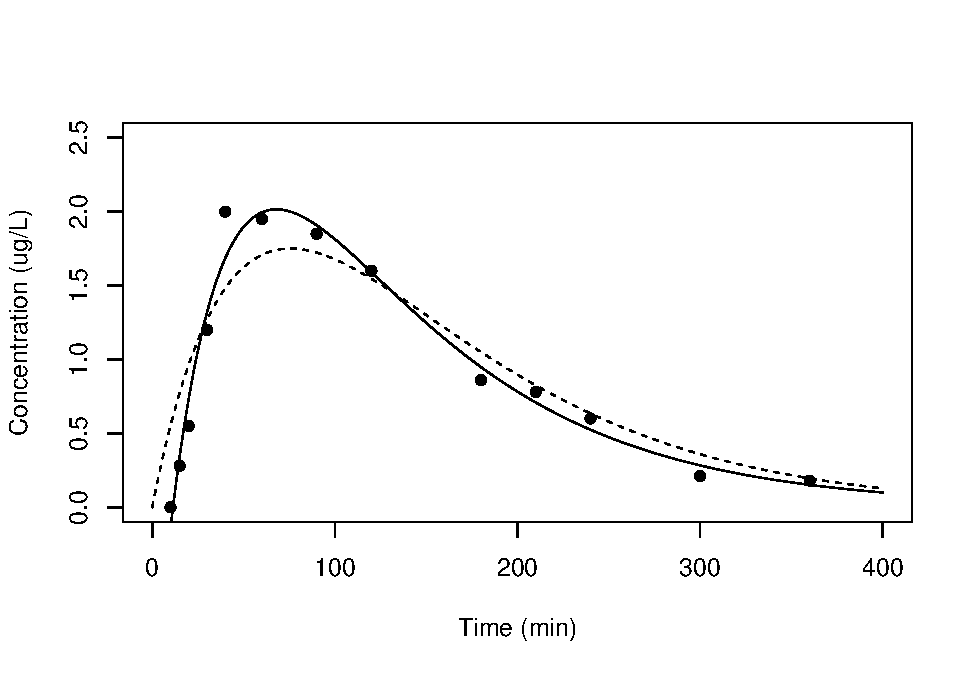
\includegraphics{handout_files/figure-latex/unnamed-chunk-5-1.pdf}

\hypertarget{one-compartment-model---iv-dosing}{%
\chapter{One compartment model - IV dosing}\label{one-compartment-model---iv-dosing}}

\texttt{wnl} 라이브러리를 불러오고 자료를 읽어옵니다. 4명의 IV 투약 후 농도 자료를 불러와 그림을 자료 탐색을 할 수 있습니다.

\begin{Shaded}
\begin{Highlighting}[]
\KeywordTok{require}\NormalTok{(wnl)}
\NormalTok{dPK01 =}\StringTok{ }\KeywordTok{read.csv}\NormalTok{(}\StringTok{"data/hands-on2.csv"}\NormalTok{, }\DataTypeTok{skip=}\DecValTok{1}\NormalTok{)}
\KeywordTok{colnames}\NormalTok{(dPK01) =}\StringTok{ }\KeywordTok{c}\NormalTok{(}\StringTok{"TIME"}\NormalTok{, }\StringTok{"DV"}\NormalTok{, }\StringTok{"ID"}\NormalTok{)}

\KeywordTok{library}\NormalTok{(ggplot2)}
\KeywordTok{ggplot}\NormalTok{(dPK01, }\KeywordTok{aes}\NormalTok{(TIME, DV, }\DataTypeTok{group =}\NormalTok{ ID, }\DataTypeTok{color =} \KeywordTok{as.factor}\NormalTok{(ID))) }\OperatorTok{+}
\StringTok{  }\KeywordTok{geom_line}\NormalTok{() }\OperatorTok{+}\StringTok{ }\KeywordTok{geom_point}\NormalTok{() }\OperatorTok{+}\StringTok{ }\KeywordTok{scale_y_log10}\NormalTok{()}
\end{Highlighting}
\end{Shaded}

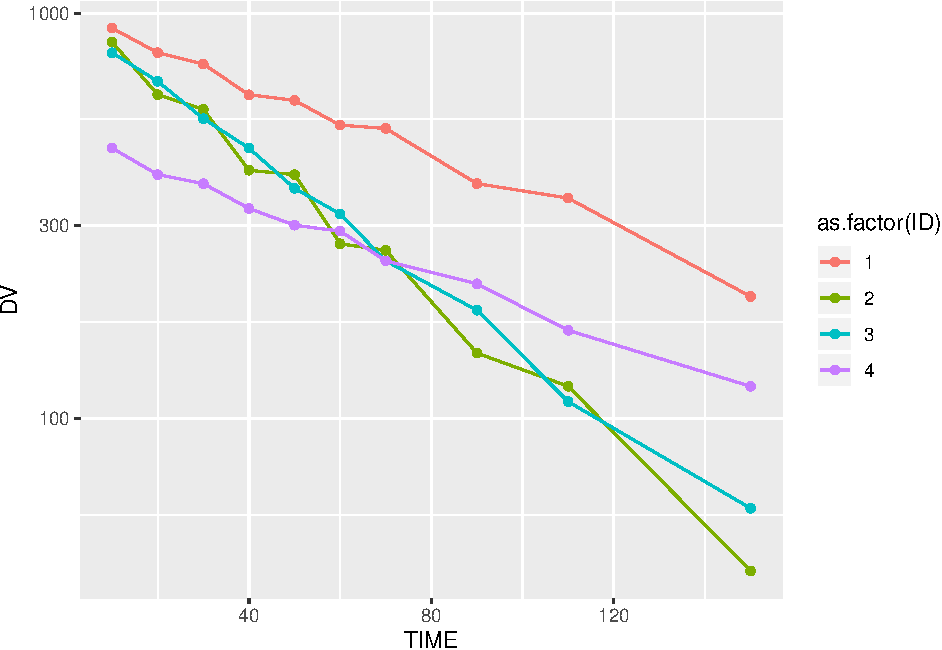
\includegraphics{handout_files/figure-latex/unnamed-chunk-6-1.pdf}

\begin{itemize}
\tightlist
\item
  4명의 피험자 모두 대략적으로 시간에 따른 농도 감소가 단항 지수함수적인 것을 관찰할 수
  있습니다.\\
\item
  피험자 1과 2를 비교하면 2번 피험자가 AUC가 더 작으며, 따라서 청소율이 더 클 것이라
  예상할 수 있으며, Y 절편이 거의 같은 것으로 보아 분포용적이 유사할 것으로 보입니다.\\
\item
  피험자 3과 4의 경우 곡선이 교차하는 형태로 눈으로는 어느 쪽이 AUC가 클지 알기 어렵고, Y절편에
  해당하는 농도가 높은 쪽이 분포용적이 더 작을 것이라 예상할 수 있습니다.
\end{itemize}

4명 자료의 NCA 분석을 \texttt{tblNCA()} 함수를 사용해 계산할 수 있습니다.

\begin{Shaded}
\begin{Highlighting}[]
\NormalTok{NonCompart}\OperatorTok{::}\KeywordTok{tblNCA}\NormalTok{(dPK01, }\DataTypeTok{key=}\StringTok{"ID"}\NormalTok{, }\DataTypeTok{colTime=}\StringTok{"TIME"}\NormalTok{, }\DataTypeTok{colConc=}\StringTok{"DV"}\NormalTok{, }\DataTypeTok{dose=}\DecValTok{10}\NormalTok{, }\DataTypeTok{adm=}\StringTok{"Bolus"}\NormalTok{)}
\end{Highlighting}
\end{Shaded}

\begin{verbatim}
##   ID       b0 CMAX CMAXD TMAX TLAG CLST     CLSTP TLST   LAMZHL
## 1  1 6.918913  920  92.0   10   NA  200 211.19414  150 66.38766
## 2  2 6.934162  850  85.0   10   NA   42  45.17696  150 33.28625
## 3  3 6.877619  800  80.0   10   NA   60  56.80923  150 36.63672
## 4  4 6.207537  465  46.5   10   NA  120 117.19292  150 72.01703
##          LAMZ LAMZLL LAMZUL LAMZNPT     CORRXY        R2     R2ADJ
## 1 0.010440904     10    150      10 -0.9943381 0.9887083 0.9872969
## 2 0.020823832     10    150      10 -0.9950967 0.9902174 0.9889946
## 3 0.018919466     10    150      10 -0.9984467 0.9968957 0.9965077
## 4 0.009624768     10    150      10 -0.9971818 0.9943716 0.9936681
##     AUCLST   AUCALL   AUCIFO  AUCIFOD   AUCIFP  AUCIFPD    AUCPEO   AUCPEP
## 1 77590.00 77590.00 96745.43 9674.543 97817.57 9781.757 19.799828 20.67887
## 2 48374.13 48374.13 50391.05 5039.105 50543.61 5054.361  4.002536  4.29230
## 3 48430.88 48430.88 51602.22 5160.222 51433.57 5143.357  6.145738  5.83799
## 4 39677.81 39677.81 52145.65 5214.565 51853.99 5185.399 23.909634 23.48167
##   AUMCLST AUMCIFO AUMCIFP  AUMCPEO  AUMCPEP        C0   AUCPBEO   AUCPBEP
## 1 4337000 9044967 9308475 52.05068 53.40805 1058.0000 10.222705 10.110658
## 2 1967000 2366394 2396605 16.87776 17.92557 1146.8254 19.813295 19.753490
## 3 2077250 2720574 2686362 23.64661 22.67423  941.1765 16.871139 16.926460
## 4 2245250 5410815 5336766 58.50441 57.92864  540.5625  9.641865  9.696095
##         VZO       VZP       CLO       CLP MRTIVLST  MRTIVIFO  MRTIVIFP
## 1  9.899914  9.791405 0.1033641 0.1022311 55.89638  93.49244  95.16158
## 2  9.529848  9.501083 0.1984480 0.1978489 40.66223  46.96061  47.41658
## 3 10.242896 10.276482 0.1937901 0.1944256 42.89102  52.72203  52.22974
## 4 19.924695 20.036761 0.1917706 0.1928492 56.58704 103.76352 102.91908
##        VSSO      VSSP
## 1  9.663758  9.728475
## 2  9.319237  9.381321
## 3 10.217007 10.154796
## 4 19.898788 19.847860
\end{verbatim}

\begin{Shaded}
\begin{Highlighting}[]
\NormalTok{IDs =}\StringTok{ }\KeywordTok{unique}\NormalTok{(dPK01[,}\StringTok{"ID"}\NormalTok{])}
\NormalTok{nID =}\StringTok{ }\KeywordTok{length}\NormalTok{(IDs)}
\NormalTok{DOSE =}\StringTok{ }\DecValTok{10000} \CommentTok{# ug}
\end{Highlighting}
\end{Shaded}

\hypertarget{compartmental-analysis}{%
\section{Compartmental analysis}\label{compartmental-analysis}}

V, K만 있으면 단항 지수함수적 농도 감소를 보이는 IV dosing의 농도를 나타낼 수 있으므로 아래와 같이 간단한 함수를 만들 수 있습니다.

\begin{Shaded}
\begin{Highlighting}[]
\NormalTok{fPK01 =}\StringTok{ }\ControlFlowTok{function}\NormalTok{(THETA) }\CommentTok{# Prediction function}
\NormalTok{\{}
\NormalTok{  V  =}\StringTok{ }\NormalTok{THETA[}\DecValTok{1}\NormalTok{]}
\NormalTok{  K  =}\StringTok{ }\NormalTok{THETA[}\DecValTok{2}\NormalTok{]}
\NormalTok{  Cp =}\StringTok{ }\NormalTok{DOSE}\OperatorTok{/}\NormalTok{V}\OperatorTok{*}\KeywordTok{exp}\NormalTok{(}\OperatorTok{-}\NormalTok{K}\OperatorTok{*}\NormalTok{TIME)  }\CommentTok{# External DOSE, TIME, eq 1:2}
  \KeywordTok{return}\NormalTok{(Cp)}
\NormalTok{\}}
\end{Highlighting}
\end{Shaded}

여러명의 자료를 분석하기 위해 \texttt{for} 함수를 사용하였습니다. 복잡해보이지만 \texttt{nlr} 함수를 사용하는 것이 핵심입니다.

\begin{Shaded}
\begin{Highlighting}[]
\NormalTok{Result =}\StringTok{ }\KeywordTok{vector}\NormalTok{()}
\ControlFlowTok{for}\NormalTok{ (i }\ControlFlowTok{in} \DecValTok{1}\OperatorTok{:}\NormalTok{nID) \{}
\NormalTok{  cID =}\StringTok{ }\NormalTok{IDs[i]}
\NormalTok{  Data =}\StringTok{ }\NormalTok{dPK01[dPK01}\OperatorTok{$}\NormalTok{ID }\OperatorTok{==}\StringTok{ }\NormalTok{cID,]}
\NormalTok{  TIME =}\StringTok{ }\NormalTok{dPK01[dPK01}\OperatorTok{$}\NormalTok{ID }\OperatorTok{==}\StringTok{ }\NormalTok{cID,}\StringTok{"TIME"}\NormalTok{]}
\NormalTok{  Res =}\StringTok{ }\KeywordTok{nlr}\NormalTok{(fPK01, Data, }\DataTypeTok{pNames=}\KeywordTok{c}\NormalTok{(}\StringTok{"V"}\NormalTok{, }\StringTok{"k"}\NormalTok{), }\DataTypeTok{IE=}\KeywordTok{c}\NormalTok{(}\DecValTok{20}\NormalTok{, }\FloatTok{0.2}\NormalTok{),}
            \DataTypeTok{SecNames=}\KeywordTok{c}\NormalTok{(}\StringTok{"CL"}\NormalTok{, }\StringTok{"AUC"}\NormalTok{, }\StringTok{"AUMC"}\NormalTok{ , }\StringTok{"Thalf"}\NormalTok{, }\StringTok{"MRT"}\NormalTok{), }
            \DataTypeTok{SecForms=}\KeywordTok{c}\NormalTok{(}\OperatorTok{~}\NormalTok{V}\OperatorTok{*}\NormalTok{k, }\OperatorTok{~}\NormalTok{DOSE}\OperatorTok{/}\NormalTok{V}\OperatorTok{/}\NormalTok{k, }\OperatorTok{~}\NormalTok{DOSE}\OperatorTok{/}\NormalTok{V}\OperatorTok{/}\NormalTok{k}\OperatorTok{/}\NormalTok{k, }\OperatorTok{~}\KeywordTok{log}\NormalTok{(}\DecValTok{2}\NormalTok{)}\OperatorTok{/}\NormalTok{k, }\OperatorTok{~}\DecValTok{1}\OperatorTok{/}\NormalTok{k))}
\NormalTok{  Result =}\StringTok{ }\KeywordTok{rbind}\NormalTok{(Result, }\KeywordTok{cbind}\NormalTok{(}\DataTypeTok{ID=}\NormalTok{cID, Res}\OperatorTok{$}\NormalTok{Est))}
\NormalTok{\} ; Result}
\end{Highlighting}
\end{Shaded}

\begin{verbatim}
##     ID          V            k AddErrVar  AddErrSD          CL
## PE   1  9.9784487 0.0102560820 432.73767 20.802348 0.102339788
## SE   1  0.1834206 0.0003873927 193.52612  4.651545 0.002597160
## RSE  1  1.8381673 3.7771994487  44.72135 22.360674 2.537781676
## PE   2  9.8162458 0.0206612797 753.97041 27.458522 0.202816199
## SE   2  0.3308035 0.0010187679 337.18516  6.139900 0.005970426
## RSE  2  3.3699589 4.9308074311  44.72127 22.360637 2.943762128
## PE   3 10.2230093 0.0190412124  77.05108  8.777874 0.194658492
## SE   3  0.1086744 0.0003052182  34.45832  1.962794 0.001891101
## RSE  3  1.0630369 1.6029348653  44.72140 22.360699 0.971496569
## PE   4 19.9471606 0.0098139570  72.19448  8.496733 0.195760575
## SE   4  0.2954327 0.0003070959  32.28660  1.899942 0.004148218
## RSE  4  1.4810766 3.1291754937  44.72170 22.360849 2.119026160
##              AUC         AUMC      Thalf        MRT
## PE  9.771371e+04 9.527391e+06 67.5840131  97.503121
## SE  2.479761e+03 5.875882e+05  2.5527830   3.682887
## RSE 2.537782e+00 6.167356e+00  3.7771994   3.777199
## PE  4.930573e+04 2.386383e+06 33.5481244  48.399713
## SE  1.451443e+03 1.763351e+05  1.6541934   2.386497
## RSE 2.943762e+00 7.389220e+00  4.9308074   4.930807
## PE  5.137202e+04 2.697939e+06 36.4024709  52.517664
## SE  4.990774e+02 6.551250e+04  0.5835079   0.841824
## RSE 9.714966e-01 2.428243e+00  1.6029349   1.602935
## PE  5.108281e+04 5.205118e+06 70.6287162 101.895699
## SE  1.082458e+03 2.672940e+05  2.2100965   3.188495
## RSE 2.119026e+00 5.135215e+00  3.1291755   3.129175
\end{verbatim}

\hypertarget{modeling-result-1}{%
\section{Modeling Result}\label{modeling-result-1}}

\begin{Shaded}
\begin{Highlighting}[]
\CommentTok{# Figure 1.1, p 470}
\KeywordTok{plot}\NormalTok{(}\DecValTok{0}\NormalTok{, }\DecValTok{1}\NormalTok{, }\DataTypeTok{type=}\StringTok{"n"}\NormalTok{, }\DataTypeTok{xlim=}\KeywordTok{c}\NormalTok{(}\DecValTok{0}\NormalTok{, }\DecValTok{160}\NormalTok{), }\DataTypeTok{ylim=}\KeywordTok{c}\NormalTok{(}\DecValTok{10}\NormalTok{, }\DecValTok{1000}\NormalTok{), }\DataTypeTok{log=}\StringTok{"y"}\NormalTok{, }\DataTypeTok{xlab=}\StringTok{"Time (min)"}\NormalTok{, }\DataTypeTok{ylab=}\StringTok{"Concentration (ug/L)"}\NormalTok{)}
\ControlFlowTok{for}\NormalTok{ (i }\ControlFlowTok{in} \DecValTok{1}\OperatorTok{:}\NormalTok{nID) \{}
\NormalTok{  cID =}\StringTok{ }\NormalTok{IDs[i]}
\NormalTok{  TIME =}\StringTok{ }\NormalTok{dPK01[dPK01}\OperatorTok{$}\NormalTok{ID }\OperatorTok{==}\StringTok{ }\NormalTok{cID,}\StringTok{"TIME"}\NormalTok{]}
  \KeywordTok{points}\NormalTok{(TIME, dPK01[dPK01}\OperatorTok{$}\NormalTok{ID }\OperatorTok{==}\StringTok{ }\NormalTok{cID,}\StringTok{"DV"}\NormalTok{], }\DataTypeTok{pch=}\DecValTok{14}\OperatorTok{+}\NormalTok{i)}
\NormalTok{  cTHETA =}\StringTok{ }\NormalTok{Result[Result[,}\StringTok{"ID"}\NormalTok{]}\OperatorTok{==}\NormalTok{cID }\OperatorTok{&}\StringTok{ }\KeywordTok{rownames}\NormalTok{(Result)}\OperatorTok{==}\StringTok{"PE"}\NormalTok{, }\KeywordTok{c}\NormalTok{(}\StringTok{"V"}\NormalTok{, }\StringTok{"k"}\NormalTok{)]}
  \KeywordTok{lines}\NormalTok{(TIME, }\KeywordTok{fPK01}\NormalTok{(cTHETA))   }
\NormalTok{\}}
\end{Highlighting}
\end{Shaded}

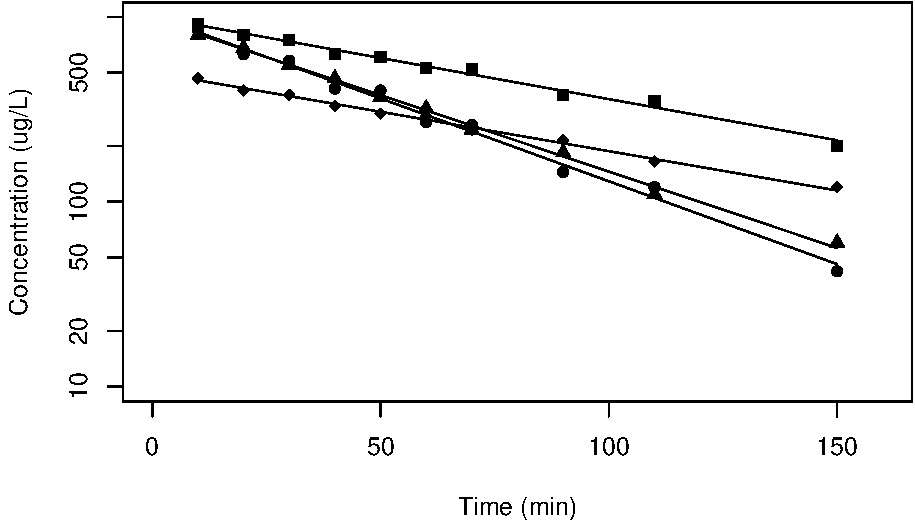
\includegraphics{handout_files/figure-latex/unnamed-chunk-10-1.pdf}

\hypertarget{two-compartment-model-oral-dosing}{%
\chapter{Two compartment model -- oral dosing}\label{two-compartment-model-oral-dosing}}

\begin{Shaded}
\begin{Highlighting}[]
\KeywordTok{require}\NormalTok{(wnl)}
\NormalTok{dPK14 =}\StringTok{ }\KeywordTok{read.csv}\NormalTok{(}\StringTok{"data-old/PK14.csv"}\NormalTok{, }\DataTypeTok{skip=}\DecValTok{1}\NormalTok{)}
\KeywordTok{colnames}\NormalTok{(dPK14) =}\StringTok{ }\KeywordTok{c}\NormalTok{(}\StringTok{"TIME"}\NormalTok{, }\StringTok{"DV"}\NormalTok{) ; dPK14}
\end{Highlighting}
\end{Shaded}

\begin{verbatim}
##      TIME     DV
## 1   0.083  13.90
## 2   0.167 152.00
## 3   0.250 226.00
## 4   0.500 204.00
## 5   1.000 149.00
## 6   1.500 100.00
## 7   2.000  66.00
## 8   3.000  36.00
## 9   4.000  17.70
## 10  6.000   6.90
## 11  8.000   3.96
## 12 12.000   2.89
## 13 24.000   0.90
## 14 25.000   0.90
\end{verbatim}

\begin{Shaded}
\begin{Highlighting}[]
\NormalTok{Dpo =}\StringTok{ }\DecValTok{23158}
\end{Highlighting}
\end{Shaded}

\hypertarget{compartmental-analysis-without-tlag-1}{%
\section{Compartmental analysis without Tlag}\label{compartmental-analysis-without-tlag-1}}

경구 투여 2구획 분석, 지연시간이 없는 모형입니다. Ka, V, k21, alpha, beta 로 농도를 나타낼 수 있습니다.

\begin{Shaded}
\begin{Highlighting}[]
\CommentTok{## without lag}
\NormalTok{fPK14a =}\StringTok{ }\ControlFlowTok{function}\NormalTok{(THETA)}
\NormalTok{\{}
\NormalTok{  Vc  =}\StringTok{ }\NormalTok{THETA[}\DecValTok{1}\NormalTok{]}
\NormalTok{  Ka  =}\StringTok{ }\NormalTok{THETA[}\DecValTok{2}\NormalTok{]}
\NormalTok{  k21 =}\StringTok{ }\NormalTok{THETA[}\DecValTok{3}\NormalTok{]}
\NormalTok{  a   =}\StringTok{ }\NormalTok{THETA[}\DecValTok{4}\NormalTok{] }\CommentTok{# alpha}
\NormalTok{  b   =}\StringTok{ }\NormalTok{THETA[}\DecValTok{5}\NormalTok{] }\CommentTok{# beta}
  
\NormalTok{  T1 =}\StringTok{ }\NormalTok{e}\OperatorTok{$}\NormalTok{DATA[,}\StringTok{"TIME"}\NormalTok{]}
\NormalTok{  Co =}\StringTok{ }\NormalTok{Ka}\OperatorTok{*}\NormalTok{Dpo}\OperatorTok{/}\NormalTok{Vc}\OperatorTok{*}\NormalTok{((k21}\OperatorTok{-}\NormalTok{a)}\OperatorTok{/}\NormalTok{(Ka}\OperatorTok{-}\NormalTok{a)}\OperatorTok{/}\NormalTok{(b}\OperatorTok{-}\NormalTok{a)}\OperatorTok{*}\KeywordTok{exp}\NormalTok{(}\OperatorTok{-}\NormalTok{a}\OperatorTok{*}\NormalTok{T1) }\OperatorTok{+}\StringTok{ }
\StringTok{                    }\NormalTok{(k21}\OperatorTok{-}\NormalTok{b)}\OperatorTok{/}\NormalTok{(Ka}\OperatorTok{-}\NormalTok{b)}\OperatorTok{/}\NormalTok{(a}\OperatorTok{-}\NormalTok{b)}\OperatorTok{*}\KeywordTok{exp}\NormalTok{(}\OperatorTok{-}\NormalTok{b}\OperatorTok{*}\NormalTok{T1) }\OperatorTok{+}\StringTok{ }
\StringTok{                    }\NormalTok{(k21}\OperatorTok{-}\NormalTok{Ka)}\OperatorTok{/}\NormalTok{(a}\OperatorTok{-}\NormalTok{Ka)}\OperatorTok{/}\NormalTok{(b}\OperatorTok{-}\NormalTok{Ka)}\OperatorTok{*}\KeywordTok{exp}\NormalTok{(}\OperatorTok{-}\NormalTok{Ka}\OperatorTok{*}\NormalTok{T1)) }\CommentTok{# Erratum in eq 14:1}
  
  \KeywordTok{return}\NormalTok{(Co)}
\NormalTok{\}}

\NormalTok{r1 <-}\StringTok{ }\KeywordTok{nlr}\NormalTok{(fPK14a, dPK14, }
          \DataTypeTok{pNames=}\KeywordTok{c}\NormalTok{(}\StringTok{"Vc/F"}\NormalTok{, }\StringTok{"Ka"}\NormalTok{, }\StringTok{"k21"}\NormalTok{, }\StringTok{"alpha"}\NormalTok{, }\StringTok{"beta"}\NormalTok{), }
          \DataTypeTok{IE=}\KeywordTok{c}\NormalTok{(}\DecValTok{350}\NormalTok{, }\DecValTok{11}\NormalTok{, }\DecValTok{1}\NormalTok{, }\FloatTok{0.1}\NormalTok{, }\FloatTok{0.01}\NormalTok{))}

\NormalTok{r1}\OperatorTok{$}\NormalTok{Est}
\end{Highlighting}
\end{Shaded}

\begin{verbatim}
##         Vc/F        Ka         k21     alpha        beta AddErrVar
## PE  43.63080  2.349584   0.6979441  2.346109   0.3973269 537.19125
## SE  40.60547  2.222099   0.9644243  2.221849   0.4937935 203.03693
## RSE 93.06606 94.574121 138.1807351 94.703582 124.2789064  37.79602
##      AddErrSD
## PE  23.177387
## SE   4.380065
## RSE 18.898011
\end{verbatim}

\hypertarget{compartmental-analysis-with-tlag-1}{%
\section{Compartmental analysis with Tlag}\label{compartmental-analysis-with-tlag-1}}

경구 투여 일구획 분석, 지연시간이 있는 모형입니다. Ka, V, k21, alpha, beta 에 Tlag가 추가되어 농도를 나타낼 수 있습니다.

\begin{Shaded}
\begin{Highlighting}[]
\CommentTok{## with lag}
\NormalTok{fPK14b =}\StringTok{ }\ControlFlowTok{function}\NormalTok{(THETA)}
\NormalTok{\{}
\NormalTok{  Vc  =}\StringTok{ }\NormalTok{THETA[}\DecValTok{1}\NormalTok{]}
\NormalTok{  Ka  =}\StringTok{ }\NormalTok{THETA[}\DecValTok{2}\NormalTok{]}
\NormalTok{  k21 =}\StringTok{ }\NormalTok{THETA[}\DecValTok{3}\NormalTok{]}
\NormalTok{  a   =}\StringTok{ }\NormalTok{THETA[}\DecValTok{4}\NormalTok{] }\CommentTok{# alpha}
\NormalTok{  b   =}\StringTok{ }\NormalTok{THETA[}\DecValTok{5}\NormalTok{] }\CommentTok{# beta}
\NormalTok{  TL  =}\StringTok{ }\NormalTok{THETA[}\DecValTok{6}\NormalTok{] }\CommentTok{# Tlag}
  
\NormalTok{  T1 =}\StringTok{ }\NormalTok{e}\OperatorTok{$}\NormalTok{DATA[,}\StringTok{"TIME"}\NormalTok{]}
\NormalTok{  Co =}\StringTok{ }\NormalTok{Ka}\OperatorTok{*}\NormalTok{Dpo}\OperatorTok{/}\NormalTok{Vc}\OperatorTok{*}\NormalTok{((k21}\OperatorTok{-}\NormalTok{a)}\OperatorTok{/}\NormalTok{(Ka}\OperatorTok{-}\NormalTok{a)}\OperatorTok{/}\NormalTok{(b}\OperatorTok{-}\NormalTok{a)}\OperatorTok{*}\KeywordTok{exp}\NormalTok{(}\OperatorTok{-}\NormalTok{a}\OperatorTok{*}\NormalTok{(T1}\OperatorTok{-}\NormalTok{TL)) }\OperatorTok{+}\StringTok{ }
\StringTok{                    }\NormalTok{(k21}\OperatorTok{-}\NormalTok{b)}\OperatorTok{/}\NormalTok{(Ka}\OperatorTok{-}\NormalTok{b)}\OperatorTok{/}\NormalTok{(a}\OperatorTok{-}\NormalTok{b)}\OperatorTok{*}\KeywordTok{exp}\NormalTok{(}\OperatorTok{-}\NormalTok{b}\OperatorTok{*}\NormalTok{(T1}\OperatorTok{-}\NormalTok{TL)) }\OperatorTok{+}\StringTok{ }
\StringTok{                    }\NormalTok{(k21}\OperatorTok{-}\NormalTok{Ka)}\OperatorTok{/}\NormalTok{(a}\OperatorTok{-}\NormalTok{Ka)}\OperatorTok{/}\NormalTok{(b}\OperatorTok{-}\NormalTok{Ka)}\OperatorTok{*}\KeywordTok{exp}\NormalTok{(}\OperatorTok{-}\NormalTok{Ka}\OperatorTok{*}\NormalTok{(T1}\OperatorTok{-}\NormalTok{TL))) }
\NormalTok{  Co[Co }\OperatorTok{<}\StringTok{ }\DecValTok{0}\NormalTok{] =}\StringTok{ }\DecValTok{0} \CommentTok{# remove negative concentrationss before tlag}
  
  \KeywordTok{return}\NormalTok{(Co)}
\NormalTok{\}}

\NormalTok{r2 <-}\StringTok{ }\KeywordTok{nlr}\NormalTok{(fPK14b, dPK14, }
          \DataTypeTok{pNames=}\KeywordTok{c}\NormalTok{(}\StringTok{"Vc/F"}\NormalTok{, }\StringTok{"Ka"}\NormalTok{, }\StringTok{"k21"}\NormalTok{, }\StringTok{"alpha"}\NormalTok{, }\StringTok{"beta"}\NormalTok{, }\StringTok{"Tlag"}\NormalTok{), }
          \DataTypeTok{IE=}\KeywordTok{c}\NormalTok{(}\DecValTok{150}\NormalTok{, }\DecValTok{11}\NormalTok{, }\FloatTok{0.12}\NormalTok{, }\FloatTok{0.1}\NormalTok{, }\FloatTok{0.01}\NormalTok{, }\FloatTok{0.05}\NormalTok{))}
\NormalTok{r2}\OperatorTok{$}\NormalTok{Est}
\end{Highlighting}
\end{Shaded}

\begin{verbatim}
##          Vc/F        Ka          k21      alpha         beta        Tlag
## PE  88.530347 19.777685    0.0079704 0.73178583 2.021746e-03 0.121649379
## SE   2.318778  3.774496    0.1245099 0.04591788 1.130516e-01 0.008133633
## RSE  2.619190 19.084619 1562.1537739 6.27477041 5.591779e+03 6.686127672
##     AddErrVar   AddErrSD
## PE  17.889619  4.2296122
## SE   6.848254  0.8095605
## RSE 38.280600 19.1403000
\end{verbatim}

\hypertarget{modeling-result-2}{%
\section{Modeling Result}\label{modeling-result-2}}

지연 시간이 있는 모형의 적합이 더 좋은 것을 알 수 있습니다. Cmax 부분을 주의깊게 살펴보세요.

\begin{Shaded}
\begin{Highlighting}[]
\KeywordTok{plot}\NormalTok{(dPK14[,}\StringTok{"TIME"}\NormalTok{], dPK14[,}\StringTok{"DV"}\NormalTok{], }\DataTypeTok{xlim=}\KeywordTok{c}\NormalTok{(}\DecValTok{0}\NormalTok{, }\DecValTok{25}\NormalTok{), }\DataTypeTok{ylim=}\KeywordTok{c}\NormalTok{(}\DecValTok{0}\NormalTok{, }\DecValTok{250}\NormalTok{), }\DataTypeTok{xlab=}\StringTok{"Time (min)"}\NormalTok{, }\DataTypeTok{ylab=}\StringTok{"Concentration (ug/L)"}\NormalTok{, }\DataTypeTok{pch=}\DecValTok{16}\NormalTok{)}
\NormalTok{TIME =}\StringTok{ }\NormalTok{dPK14[,}\StringTok{"TIME"}\NormalTok{]}
\KeywordTok{lines}\NormalTok{(TIME, }\KeywordTok{fPK14a}\NormalTok{(r1}\OperatorTok{$}\NormalTok{Est[}\StringTok{"PE"}\NormalTok{, }\DecValTok{1}\OperatorTok{:}\DecValTok{5}\NormalTok{]), }\DataTypeTok{lty=}\DecValTok{2}\NormalTok{)}
\KeywordTok{lines}\NormalTok{(TIME, }\KeywordTok{fPK14b}\NormalTok{(r2}\OperatorTok{$}\NormalTok{Est[}\StringTok{"PE"}\NormalTok{, }\DecValTok{1}\OperatorTok{:}\DecValTok{6}\NormalTok{]))}
\end{Highlighting}
\end{Shaded}

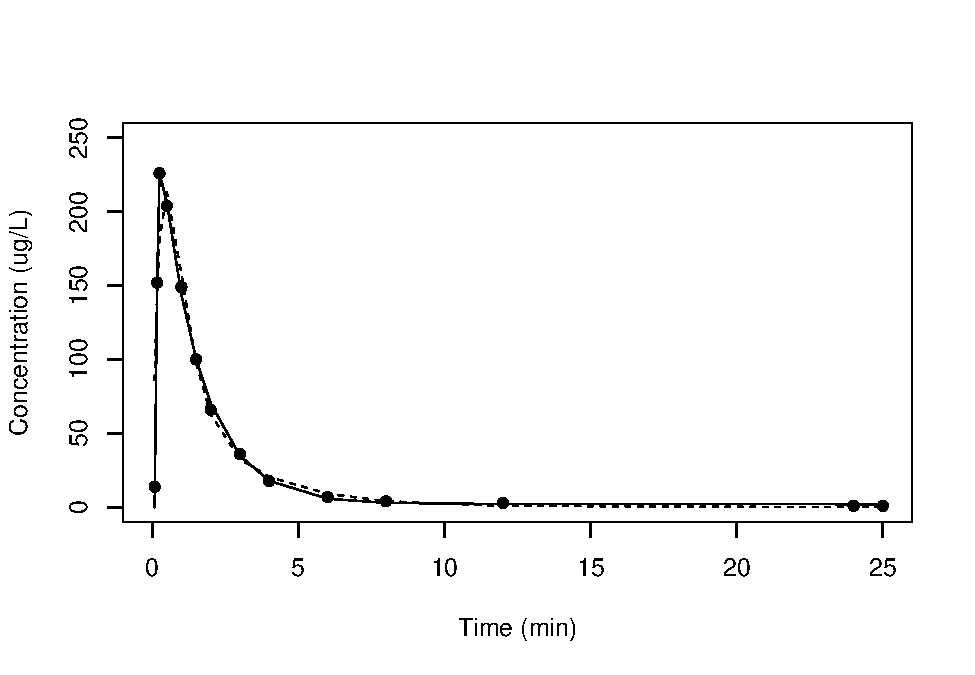
\includegraphics{handout_files/figure-latex/unnamed-chunk-14-1.pdf}

\hypertarget{refs}{}
\leavevmode\hypertarget{ref-R-wnl}{}%
Bae, Kyun-Seop. 2018. \emph{Wnl: Minimization Tool for Pharmacokinetic-Pharmacodynamic Data Analysis}. \url{https://CRAN.R-project.org/package=wnl}.

\leavevmode\hypertarget{ref-gab}{}%
Gabrielsson, Johan. 2016. \emph{Pharmacokinetic and Pharmacodynamic Data Analysis : Concepts and Applications}. Stockholm: Apotekarsocieteten.

\end{document}
